
%% bare_conf_compsoc.tex
%% V1.4b
%% 2015/08/26
%% by Michael Shell
%% See:
%% http://www.michaelshell.org/
%% for current contact information.
%%
%% This is a skeleton file demonstrating the use of IEEEtran.cls
%% (requires IEEEtran.cls version 1.8b or later) with an IEEE Computer
%% Society conference paper.
%%
%% Support sites:
%% http://www.michaelshell.org/tex/ieeetran/
%% http://www.ctan.org/pkg/ieeetran
%% and
%% http://www.ieee.org/

%%*************************************************************************
%% Legal Notice:
%% This code is offered as-is without any warranty either expressed or
%% implied; without even the implied warranty of MERCHANTABILITY or
%% FITNESS FOR A PARTICULAR PURPOSE! 
%% User assumes all risk.
%% In no event shall the IEEE or any contributor to this code be liable for
%% any damages or losses, including, but not limited to, incidental,
%% consequential, or any other damages, resulting from the use or misuse
%% of any information contained here.
%%
%% All comments are the opinions of their respective authors and are not
%% necessarily endorsed by the IEEE.
%%
%% This work is distributed under the LaTeX Project Public License (LPPL)
%% ( http://www.latex-project.org/ ) version 1.3, and may be freely used,
%% distributed and modified. A copy of the LPPL, version 1.3, is included
%% in the base LaTeX documentation of all distributions of LaTeX released
%% 2003/12/01 or later.
%% Retain all contribution notices and credits.
%% ** Modified files should be clearly indicated as such, including  **
%% ** renaming them and changing author support contact information. **
%%*************************************************************************


% *** Authors should verify (and, if needed, correct) their LaTeX system  ***
% *** with the testflow diagnostic prior to trusting their LaTeX platform ***
% *** with production work. The IEEE's font choices and paper sizes can   ***
% *** trigger bugs that do not appear when using other class files.       ***                          ***
% The testflow support page is at:
% http://www.michaelshell.org/tex/testflow/



\documentclass[conference,compsoc]{IEEEtran}
% Some/most Computer Society conferences require the compsoc mode option,
% but others may want the standard conference format.
%
% If IEEEtran.cls has not been installed into the LaTeX system files,
% manually specify the path to it like:
% \documentclass[conference,compsoc]{../sty/IEEEtran}

\usepackage{algorithm,algorithmic}
\usepackage{graphicx}
\graphicspath{ {images/} }


% Some very useful LaTeX packages include:
% (uncomment the ones you want to load)


% *** MISC UTILITY PACKAGES ***
%
%\usepackage{ifpdf}
% Heiko Oberdiek's ifpdf.sty is very useful if you need conditional
% compilation based on whether the output is pdf or dvi.
% usage:
% \ifpdf
%   % pdf code
% \else
%   % dvi code
% \fi
% The latest version of ifpdf.sty can be obtained from:
% http://www.ctan.org/pkg/ifpdf
% Also, note that IEEEtran.cls V1.7 and later provides a builtin
% \ifCLASSINFOpdf conditional that works the same way.
% When switching from latex to pdflatex and vice-versa, the compiler may
% have to be run twice to clear warning/error messages.






% *** CITATION PACKAGES ***
%
\ifCLASSOPTIONcompsoc
  % IEEE Computer Society needs nocompress option
  % requires cite.sty v4.0 or later (November 2003)
  \usepackage[nocompress]{cite}
\else
  % normal IEEE
  \usepackage{cite}
\fi
% cite.sty was written by Donald Arseneau
% V1.6 and later of IEEEtran pre-defines the format of the cite.sty package
% \cite{} output to follow that of the IEEE. Loading the cite package will
% result in citation numbers being automatically sorted and properly
% "compressed/ranged". e.g., [1], [9], [2], [7], [5], [6] without using
% cite.sty will become [1], [2], [5]--[7], [9] using cite.sty. cite.sty's
% \cite will automatically add leading space, if needed. Use cite.sty's
% noadjust option (cite.sty V3.8 and later) if you want to turn this off
% such as if a citation ever needs to be enclosed in parenthesis.
% cite.sty is already installed on most LaTeX systems. Be sure and use
% version 5.0 (2009-03-20) and later if using hyperref.sty.
% The latest version can be obtained at:
% http://www.ctan.org/pkg/cite
% The documentation is contained in the cite.sty file itself.
%
% Note that some packages require special options to format as the Computer
% Society requires. In particular, Computer Society  papers do not use
% compressed citation ranges as is done in typical IEEE papers
% (e.g., [1]-[4]). Instead, they list every citation separately in order
% (e.g., [1], [2], [3], [4]). To get the latter we need to load the cite
% package with the nocompress option which is supported by cite.sty v4.0
% and later.





% *** GRAPHICS RELATED PACKAGES ***
%
\ifCLASSINFOpdf
  % \usepackage[pdftex]{graphicx}
  % declare the path(s) where your graphic files are
  % \graphicspath{{../pdf/}{../jpeg/}}
  % and their extensions so you won't have to specify these with
  % every instance of \includegraphics
  % \DeclareGraphicsExtensions{.pdf,.jpeg,.png}
\else
  % or other class option (dvipsone, dvipdf, if not using dvips). graphicx
  % will default to the driver specified in the system graphics.cfg if no
  % driver is specified.
  % \usepackage[dvips]{graphicx}
  % declare the path(s) where your graphic files are
  % \graphicspath{{../eps/}}
  % and their extensions so you won't have to specify these with
  % every instance of \includegraphics
  % \DeclareGraphicsExtensions{.eps}
\fi
% graphicx was written by David Carlisle and Sebastian Rahtz. It is
% required if you want graphics, photos, etc. graphicx.sty is already
% installed on most LaTeX systems. The latest version and documentation
% can be obtained at: 
% http://www.ctan.org/pkg/graphicx
% Another good source of documentation is "Using Imported Graphics in
% LaTeX2e" by Keith Reckdahl which can be found at:
% http://www.ctan.org/pkg/epslatex
%
% latex, and pdflatex in dvi mode, support graphics in encapsulated
% postscript (.eps) format. pdflatex in pdf mode supports graphics
% in .pdf, .jpeg, .png and .mps (metapost) formats. Users should ensure
% that all non-photo figures use a vector format (.eps, .pdf, .mps) and
% not a bitmapped formats (.jpeg, .png). The IEEE frowns on bitmapped formats
% which can result in "jaggedy"/blurry rendering of lines and letters as
% well as large increases in file sizes.
%
% You can find documentation about the pdfTeX application at:
% http://www.tug.org/applications/pdftex





% *** MATH PACKAGES ***
%
%\usepackage{amsmath}
% A popular package from the American Mathematical Society that provides
% many useful and powerful commands for dealing with mathematics.
%
% Note that the amsmath package sets \interdisplaylinepenalty to 10000
% thus preventing page breaks from occurring within multiline equations. Use:
%\interdisplaylinepenalty=2500
% after loading amsmath to restore such page breaks as IEEEtran.cls normally
% does. amsmath.sty is already installed on most LaTeX systems. The latest
% version and documentation can be obtained at:
% http://www.ctan.org/pkg/amsmath





% *** SPECIALIZED LIST PACKAGES ***
%
%\usepackage{algorithmic}
% algorithmic.sty was written by Peter Williams and Rogerio Brito.
% This package provides an algorithmic environment fo describing algorithms.
% You can use the algorithmic environment in-text or within a figure
% environment to provide for a floating algorithm. Do NOT use the algorithm
% floating environment provided by algorithm.sty (by the same authors) or
% algorithm2e.sty (by Christophe Fiorio) as the IEEE does not use dedicated
% algorithm float types and packages that provide these will not provide
% correct IEEE style captions. The latest version and documentation of
% algorithmic.sty can be obtained at:
% http://www.ctan.org/pkg/algorithms
% Also of interest may be the (relatively newer and more customizable)
% algorithmicx.sty package by Szasz Janos:
% http://www.ctan.org/pkg/algorithmicx




% *** ALIGNMENT PACKAGES ***
%
%\usepackage{array}
% Frank Mittelbach's and David Carlisle's array.sty patches and improves
% the standard LaTeX2e array and tabular environments to provide better
% appearance and additional user controls. As the default LaTeX2e table
% generation code is lacking to the point of almost being broken with
% respect to the quality of the end results, all users are strongly
% advised to use an enhanced (at the very least that provided by array.sty)
% set of table tools. array.sty is already installed on most systems. The
% latest version and documentation can be obtained at:
% http://www.ctan.org/pkg/array


% IEEEtran contains the IEEEeqnarray family of commands that can be used to
% generate multiline equations as well as matrices, tables, etc., of high
% quality.




% *** SUBFIGURE PACKAGES ***
%\ifCLASSOPTIONcompsoc
%  \usepackage[caption=false,font=footnotesize,labelfont=sf,textfont=sf]{subfig}
%\else
%  \usepackage[caption=false,font=footnotesize]{subfig}
%\fi
% subfig.sty, written by Steven Douglas Cochran, is the modern replacement
% for subfigure.sty, the latter of which is no longer maintained and is
% incompatible with some LaTeX packages including fixltx2e. However,
% subfig.sty requires and automatically loads Axel Sommerfeldt's caption.sty
% which will override IEEEtran.cls' handling of captions and this will result
% in non-IEEE style figure/table captions. To prevent this problem, be sure
% and invoke subfig.sty's "caption=false" package option (available since
% subfig.sty version 1.3, 2005/06/28) as this is will preserve IEEEtran.cls
% handling of captions.
% Note that the Computer Society format requires a sans serif font rather
% than the serif font used in traditional IEEE formatting and thus the need
% to invoke different subfig.sty package options depending on whether
% compsoc mode has been enabled.
%
% The latest version and documentation of subfig.sty can be obtained at:
% http://www.ctan.org/pkg/subfig




% *** FLOAT PACKAGES ***
%
%\usepackage{fixltx2e}
% fixltx2e, the successor to the earlier fix2col.sty, was written by
% Frank Mittelbach and David Carlisle. This package corrects a few problems
% in the LaTeX2e kernel, the most notable of which is that in current
% LaTeX2e releases, the ordering of single and double column floats is not
% guaranteed to be preserved. Thus, an unpatched LaTeX2e can allow a
% single column figure to be placed prior to an earlier double column
% figure.
% Be aware that LaTeX2e kernels dated 2015 and later have fixltx2e.sty's
% corrections already built into the system in which case a warning will
% be issued if an attempt is made to load fixltx2e.sty as it is no longer
% needed.
% The latest version and documentation can be found at:
% http://www.ctan.org/pkg/fixltx2e


%\usepackage{stfloats}
% stfloats.sty was written by Sigitas Tolusis. This package gives LaTeX2e
% the ability to do double column floats at the bottom of the page as well
% as the top. (e.g., "\begin{figure*}[!b]" is not normally possible in
% LaTeX2e). It also provides a command:
%\fnbelowfloat
% to enable the placement of footnotes below bottom floats (the standard
% LaTeX2e kernel puts them above bottom floats). This is an invasive package
% which rewrites many portions of the LaTeX2e float routines. It may not work
% with other packages that modify the LaTeX2e float routines. The latest
% version and documentation can be obtained at:
% http://www.ctan.org/pkg/stfloats
% Do not use the stfloats baselinefloat ability as the IEEE does not allow
% \baselineskip to stretch. Authors submitting work to the IEEE should note
% that the IEEE rarely uses double column equations and that authors should try
% to avoid such use. Do not be tempted to use the cuted.sty or midfloat.sty
% packages (also by Sigitas Tolusis) as the IEEE does not format its papers in
% such ways.
% Do not attempt to use stfloats with fixltx2e as they are incompatible.
% Instead, use Morten Hogholm'a dblfloatfix which combines the features
% of both fixltx2e and stfloats:
%
% \usepackage{dblfloatfix}
% The latest version can be found at:
% http://www.ctan.org/pkg/dblfloatfix




% *** PDF, URL AND HYPERLINK PACKAGES ***
%
%\usepackage{url}
% url.sty was written by Donald Arseneau. It provides better support for
% handling and breaking URLs. url.sty is already installed on most LaTeX
% systems. The latest version and documentation can be obtained at:
% http://www.ctan.org/pkg/url
% Basically, \url{my_url_here}.




% *** Do not adjust lengths that control margins, column widths, etc. ***
% *** Do not use packages that alter fonts (such as pslatex).         ***
% There should be no need to do such things with IEEEtran.cls V1.6 and later.
% (Unless specifically asked to do so by the journal or conference you plan
% to submit to, of course. )


% correct bad hyphenation here
\hyphenation{op-tical net-works semi-conduc-tor}


\begin{document}
%
% paper title
% Titles are generally capitalized except for words such as a, an, and, as,
% at, but, by, for, in, nor, of, on, or, the, to and up, which are usually
% not capitalized unless they are the first or last word of the title.
% Linebreaks \\ can be used within to get better formatting as desired.
% Do not put math or special symbols in the title.
\title{House Price Prediction\\ CIS 572 Machine Learning Term Project - Winter 2017}


% author names and affiliations
% use a multiple column layout for up to three different
% affiliations
\author{\IEEEauthorblockN{Manujinda Wathugala}
\IEEEauthorblockA{manu@cs.uoregon.edu}
\and
\IEEEauthorblockN{Mohsina Zaman}
\IEEEauthorblockA{mzaman@cs.uoregon.edu}
\and
\IEEEauthorblockN{Himani Chawla}
\IEEEauthorblockA{himanic@cs.uoregon.edu}}

% conference papers do not typically use \thanks and this command
% is locked out in conference mode. If really needed, such as for
% the acknowledgment of grants, issue a \IEEEoverridecommandlockouts
% after \documentclass

% for over three affiliations, or if they all won't fit within the width
% of the page (and note that there is less available width in this regard for
% compsoc conferences compared to traditional conferences), use this
% alternative format:
% 
%\author{\IEEEauthorblockN{Michael Shell\IEEEauthorrefmark{1},
%Homer Simpson\IEEEauthorrefmark{2},
%James Kirk\IEEEauthorrefmark{3}, 
%Montgomery Scott\IEEEauthorrefmark{3} and
%Eldon Tyrell\IEEEauthorrefmark{4}}
%\IEEEauthorblockA{\IEEEauthorrefmark{1}School of Electrical and Computer Engineering\\
%Georgia Institute of Technology,
%Atlanta, Georgia 30332--0250\\ Email: see http://www.michaelshell.org/contact.html}
%\IEEEauthorblockA{\IEEEauthorrefmark{2}Twentieth Century Fox, Springfield, USA\\
%Email: homer@thesimpsons.com}
%\IEEEauthorblockA{\IEEEauthorrefmark{3}Starfleet Academy, San Francisco, California 96678-2391\\
%Telephone: (800) 555--1212, Fax: (888) 555--1212}
%\IEEEauthorblockA{\IEEEauthorrefmark{4}Tyrell Inc., 123 Replicant Street, Los Angeles, California 90210--4321}}




% use for special paper notices
%\IEEEspecialpapernotice{(Invited Paper)}




% make the title area
\maketitle

% As a general rule, do not put math, special symbols or citations
% in the abstract
\begin{abstract}
The focus of this study is to find the best way to predict the sale price of a house based on 79 features that describe a house. We tested several simple regression models. The major contribution of the study is researching with a novel idea to combine a classification model with a regression model and observing whether the performance improves. Although we were successful in building a model capable of combining a classifier and a regressor into a single model, the final model did not outperform the best simple models we tested.
\end{abstract}

% no keywords




% For peer review papers, you can put extra information on the cover
% page as needed:
% \ifCLASSOPTIONpeerreview
% \begin{center} \bfseries EDICS Category: 3-BBND \end{center}
% \fi
%
% For peerreview papers, this IEEEtran command inserts a page break and
% creates the second title. It will be ignored for other modes.
\IEEEpeerreviewmaketitle



\section{Introduction}
This is a regression project which aims at predicting the sale price of a house given an array of attributes about a house. The dataset we chose to work with is the "House Prices: Advanced Regression Techniques" dataset available in Kaggle.

\subsection{Dataset}
\par
The dataset contains 79 features regarding 1460 homes in Ames, Iowa, labeled with the sale price of each property. Sale prices are from year 2006 to 2010. Available features are both nominal and numerical.

\par
There are 44 nominal features and 19 numerical features. We categorized 16 features as ordinal, which include Likert scales, counts, years and months.

\par
By observing the data, we realized that value "NA" has been used to denote two things in the dataset. The 1\textsuperscript{st} usage is to notify a missing value. The other usage is to signal the unavailability of some option such as a garage in a particular home. So, we had to practice caution in interpreting the "NA" values in the data by taking into account which column "NA" appears in.

\subsubsection{Handling Missing Values}
\par
Attributes "MasVnrArea", "LotFrontage", "MasVnrType" and "Electrical" had missing values in the training dataset. For numerical columns we used the column mean and for others we used the column mode as the filler for the missing values.

\par
During testing, we realized that test data had missing values in other columns not mentioned above. We treated them the same way as we did with the training data. All the fillers were calculated only based on the training data.

\section{Methodology}
\subsection{Feature Selection \& Manipulation}
\label{sec:feature selection}
\subsubsection{Feature Selection}
\par
Based on our training data observations, we tried two kinds of feature selections. The methods of the feature selection are as follows:

\begin{enumerate} 
\par 
\item We observed that a few attributes had the same value for more than 1400 examples. Since these attributes are almost homogeneous, we surmised that they have low predictive power on the sale price. Therefore, we decided to drop these attributes in order to reduce the dimensionality of the dataset. In subsequent sections, we refer to this set of reduced features as Reduced Features. 

\par
\item We also wanted to investigate the predictive power of attributes on the sale price. Therefore, we computed the correlation coefficient of each nominal and ordinal attribute in relation to the sale price. From the computation, we observed there were several attributes with high correlation correlation. As a result, we decided to set a Threshold of 0.1 and use the features with a correlation coefficient greater than the threshold. We will refer to this set of features as Thresholded Features.
\end{enumerate}

\par
We built models on each set of features (All attributes, Reduced Features set and Thresholded Feature set) and compared the results.

\subsubsection{Feature Manipulation}
\begin{itemize}  
\par
\item \textit{Normalization: } The dataset has several different types of attributes with values with varying ranges, which might cause these attributes to dominate the prediction decision. Therefore, we decided to use min-max normalization to ensure that all attributes equally contribute to the decision in the absence of weights.
\par
\item \textit{Encoding: } As nominal attributes do not display an inherent order, using them in regression without any encoding is meaningless as distance calculation is not possible. Therefore, we decided to use OneHotEncoding to encode the nominal attributes.  
\par
\item \textit{SalePrice Transformation: } We also observed the SalePrice in the training data to be positively skewed (Fig. \ref{fig:SalePriceDist}), as there are few houses in the higher price ranges. Therefore, we used log transformation on the SalePrice to account for the skew.  
\end{itemize}

\begin{figure}[!h]
  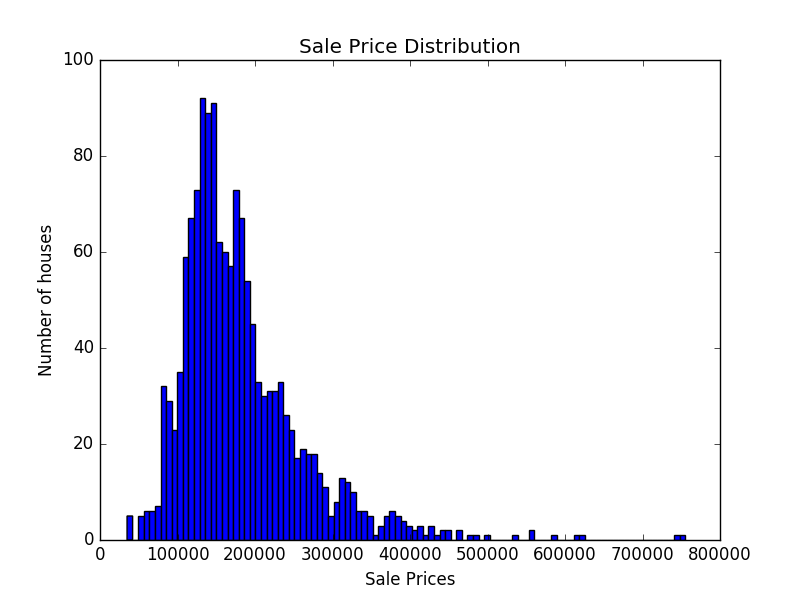
\includegraphics[width=\linewidth,natwidth=800,natheight=600]{Bins_100.png}
  \caption{Distribution of sale price}
  \label{fig:SalePriceDist}
\end{figure}

\subsection{Models Built}
\par
We decided to try and compare several different regression models and a combination of classification and regression models. The models we tried are as follows:

\begin{enumerate}  
\par
\item \textit{Regressor Models: } We tried several regression models on the different feature sets. The regression models we tried are Lasso, ADABoost, Nearest Neighbor, Random Forest, Linear and Gradient Boosting regressor.

\par
\item\textit{Classifier and Regressor Combination: } We also implemented a novel model which used a classifier to bin the dataset and a regressor to predict on each bin. For this model also, we tried different classifier and regressor combinations and compared the error for each. We refer to this model as the Custom model.

\par 
\end{enumerate} 

\subsubsection{Model Validation:} 
\par
As the dataset is small, a reserved validation set greatly reduces our training dataset size. Therefore, we employed standard 5-fold cross validation to train the basic models. However, the Custom model required us to come up with our own variation of 5-fold cross validation, which we elaborate on in the Validation section.

\section{Experiments}
\subsection{Regression Models}

\begin{table*}[!htbp]
\centering
\caption{Validation Error - Different Models Vs. Different Feature Sets}
\label{table:reg_models1}
\begin{tabular}{llll}
                          & All Attributes & Correlated + Nominal & Reduced Columns \\
GradientBoostingRegressor & 16118.18       & 16669.75           & 16256.96        \\
RandomForestRegressor     & 18906.08       & 19091.70           & 18961.65        \\
AdaBoostRegressor         & 22904.15       & 22974.78           & 22861.48        \\
%LinearRegression          & 18657.80       & 19030.90           & 18910.43        \\
%Lasso                     & 30170.24       & 30138.92           & 30139.63        \\
%SVR,(kernel = 'rbf')      & 55954.06       & 55954.22           & 55954.23        \\
                          &                &                    &                
\end{tabular}
\end{table*}

\begin{table*}[!htbp]
\centering
\caption{Validation Error - Different Models Vs. Different Numeric \& Ordinal Feature Sets}
\label{table:reg_models2}
\begin{tabular}{llll}
                      & All Attributes  & Correlated + Numeric  & Reduced, Columns \\
LinearRegression      & 19430.39        & 20851.57            & 19963.10 \\
Lasso                 & 30170.06        & 30138.92            & 30139.63 \\
SVR,(kernel = 'rbf')  & 55954.24        & 55954.39            & 55954.31 \\
\end{tabular}
\end{table*}



As a starting point, we tried different regression models to see how close we can predict without a lot of effort (Table. \ref{table:reg_models1} and Table. \ref{table:reg_models2}). We used Mean Absolute Error (MAE) to compare models since it provides a general idea about how deviated our predictions are from the actual sale price. All the reported errors are the average of five runs of 5-fold cross validation errors per each model. However, when using linear regression, lasso and SVR with RBF kernel we were unable to use the nominal attributes.

\par
For these models we obtained the least error with Gradient Boosting Regressor when using all the features (Fig. \ref{fig:gradientboosting}). The worst error was reported for SVR with RBF kernel, which suggests that the problem is more linear. Even while using only the numeric and ordinal features, the performance of linear regression is comparable to the ensemble models (Fig. \ref{fig:linearregpred}).

\begin{figure}[!h]
  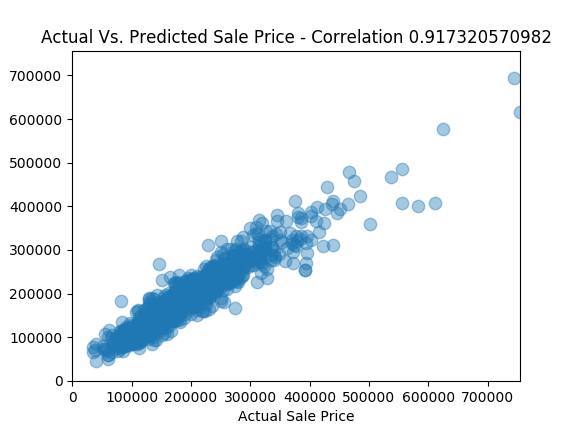
\includegraphics[width=\linewidth,natwidth=661,natheight=476]{Linear.png}
  \caption{Gradient Boosting Regression - Actual vs. Predicted Sale Price}
  \label{fig:gradientboosting}
\end{figure}

\begin{figure}[!h]
  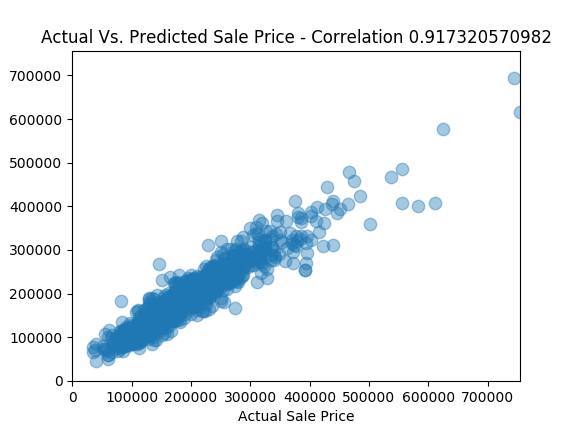
\includegraphics[width=\linewidth,natwidth=578,natheight=428]{Linear.png}
  \caption{Linear Regression - Actual vs. Predicted Sale Price}
  \label{fig:linearregpred}
\end{figure}

%\par
%To investigate which features are more important, we employed two strategies:

%\begin{enumerate}  
%\item We removed all the attributes which had a single value for more than 1400 examples out of the total 1460 training examples ("Reduced Columns" column of Table \ref{table:reg_models}). 

%\item We computed the correlation coefficient between all the numeric and ordinal with the sale price. Then we removed all the attributes which had a correlation less than 0.1 ("Correlated + Nominal" column of Table \ref{table:reg_models}).
%\end{enumerate} 

\par
We trained the same set of regressors with the two sets of reduced features. However, it caused the error to increase. Gradient Boosting, Random Forest and ADA Boost regressors perform some random feature selection while fitting the model to add diversity to the ensemble of models. This randomness gives them the chance to have better models within the ensemble and this is why they outperform Linear and Lasso regressors. 

\par
SVR with RBF kernel performed the worst and it suggests that the prediction problem at hand is more linear. However, since ensemble models, which do not fit a linear model, outperforming normal regression models suggests that attempting to fit a single linear model to the entire sale price range too is not a good idea.

\par
Moreover, since to train Linear and Lasso regressions, we only used a subset of available features (numeric and ordinal), comparing their predictions with the ensemble models which use all of the available features is unfair.

\subsection{Research Questions}
Our initial investigation made us curious about two research questions:

\begin{enumerate}  
\item Can we build a model which could make use of nominal features while using Linear or Lasso regression to predict sale prices?

\item If such a model is feasible, would it outperform or work on par with ensemble models?
\end{enumerate} 
\par
Thinking along these research questions led us towards inventing our custom model, which pipelines a classifier that classifies each house into a sale price range and a sequence of Linear or Lasso regressors that try to predict sale price within the bins. Custom Model subsection dives deep into our custom model and the experience we had with it.


\subsection{Custom Model}


\par
Standard regression models work better with numerical attributes. Although, classification models such as decision trees are initially designed to work with nominal features, the algorithms are extended to work with numeric data too. Since, the dataset has nominal, categorical and ordinal attributes, we attempted experimenting with a novel idea which matches groups of each attributes of each type with the models that work well with such attribute types.

\subsubsection{Basic idea:} 
\par
The model combines a classifier and a regressor. The classifier classifies each example into a sale price range, which is represented by a bin. Then a regression model is used to predict the actual sale price of the example with finer granularity within the bin by employing a regression model trained for that bin.

\subsubsection{Hypothesis:} 

\begin{algorithm}
\caption{Algorithm for training custom model}
\begin{algorithmic}[1]
\renewcommand{\algorithmicrequire}{\textbf{Input:}}
\renewcommand{\algorithmicensure}{\textbf{Output:}}
\REQUIRE folds, maxbins
\ENSURE  least\_error, best\_no\_of\_bins
\STATE least\_error = maxint
\STATE best\_no\_of\_bins = 0
\FOR {$bins = 1$ to $maxbins$}
  \STATE Assign bin labels to examples
  \STATE Randomly partition examples in each bin to folds (let partition f of bin b as $F_{bf}$)
  \STATE model\_fold = 0
  \FOR {$f = 1$ to $folds$}
      \STATE validation\_set = $\sum_{b=1}^{bins} F_{bf}$
      \STATE training\_set = $\sum_{b=1, i\neq f}^{bins} F_{bi}$
      \STATE Train $classifier$ on training\_set
      \STATE Validate $classifier$ on validation\_set
      \STATE Assign predicted bin labels to validation\_set examples
      \STATE Divide validation\_set based on bin labels (let validation set for bin b be $V_{b}$)
      \STATE error\_fold = 0

      \FOR {$b = 1$ to $bins$}
          \STATE regressor\_training\_set = $\sum_{i\neq f} F_{bi}$
          \STATE Train $regressor_{b}$ on regressor\_training\_set
          \STATE Validate $regressor_{b}$ on $F_{bf}$
          \STATE model\_error = Validate custom model on $V_{b}$
          \STATE error\_fold $\leftarrow$ error\_fold + model\_error
      \ENDFOR
  \ENDFOR
  \STATE model\_error $\leftarrow \frac{model\_error}{folds}$
  \IF {model\_error $\leq$ least\_error}
      \STATE least\_error = model\_error
      \STATE best\_no\_of\_bins = bins
  \ELSE
      \RETURN least\_error, best\_no\_of\_bins
  \ENDIF
\ENDFOR
\end{algorithmic} 
\end{algorithm}



\par
At the regression end, the number of bins is inversely proportional to the variation among sale prices that fall within one bin (as number of examples within a bin also decreases), which leads to a better sale price prediction. Furthermore, since the distribution of the sale prices are skewed, trying to fit a single regression model to the full range might not work well. In this light, fitting several regression models to different ranges of sale prices would provide a piecewise approximation to the sale price prediction which could outperform the single model.
However, on the classification side, the number of bins is proportional to the number of classes to predict, which leads to higher classification error.

\par
Therefore, we surmise, there should be an optimum number of bins which balances the bin classification error and the regression prediction error, and consequently minimizes the combined model error. This makes the number of bins a hyper parameter of this novel custom model. 

\subsubsection{Training:} 

\par
Based on our hypothesis, we expect the validation error to initially reduce and then start to grow as the number of bins increase further. Thus, to find the optimum number of bins, we trained multiple versions of our model increasing the number of bins from 1 to a maximum number. While this training is going on, we keep track of the validation error and watch for the moment it starts going up. We keep note of the number of bins that gave the minimum validation error thus far. Note here that we do not pick the number of bins which results in the minimum error for the whole training run, but the first bin after which the error starts growing. Choosing the number of bins that gives minimum error for the entire run quite possibly results due to over-fitting the data.

\par
Partitioning the data to perform 5-fold cross validation while training the custom model should be done with extra care. On one hand, if we use standard cross validation to train both the classifier and the array of regressors at once, we run the risk of some bins being empty or having few training (or validation) samples during training (or validation) due to the effect of random sampling. This greatly affects the training (or validation) of the regression models. On the other hand, if we train classifier and regression models separately using 5-fold classification, we have to use the validation set of the classifier as the validation set for the full model. This is error-prone since the regression models could have seen some of these held out data because the held out validation sets for classification and regression models are computed independent of each other.

\par
As the first step to reduce the risk of training (or validation) data sparsity for some regression models, we decided to use equal frequency binning to assign a bin label for each example. This makes sure that each regression model initially has a similar number of examples to train on. Making sure that we have an uncontaminated validation set throughout the training process took more effort (Algorithm 1).

\begin{figure}[!h]
  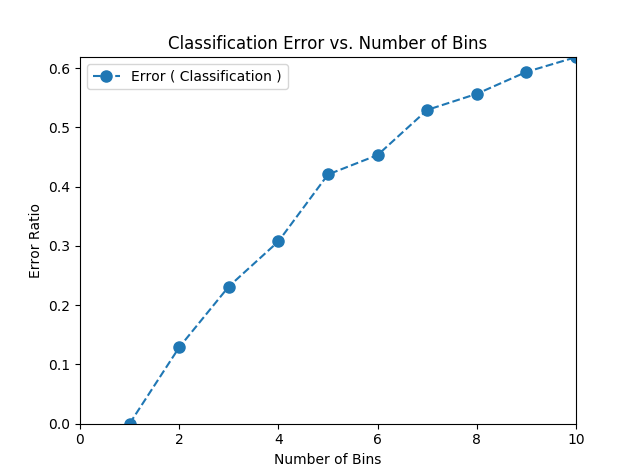
\includegraphics[width=\linewidth,natwidth=640,natheight=476]{DT_Linear_binerror.png}
  \caption{Custom Model Training - Classification Errors vs. Number of Bins}
  \label{fig:classificatinerror}
\end{figure}

\begin{figure*}[!htbp]
  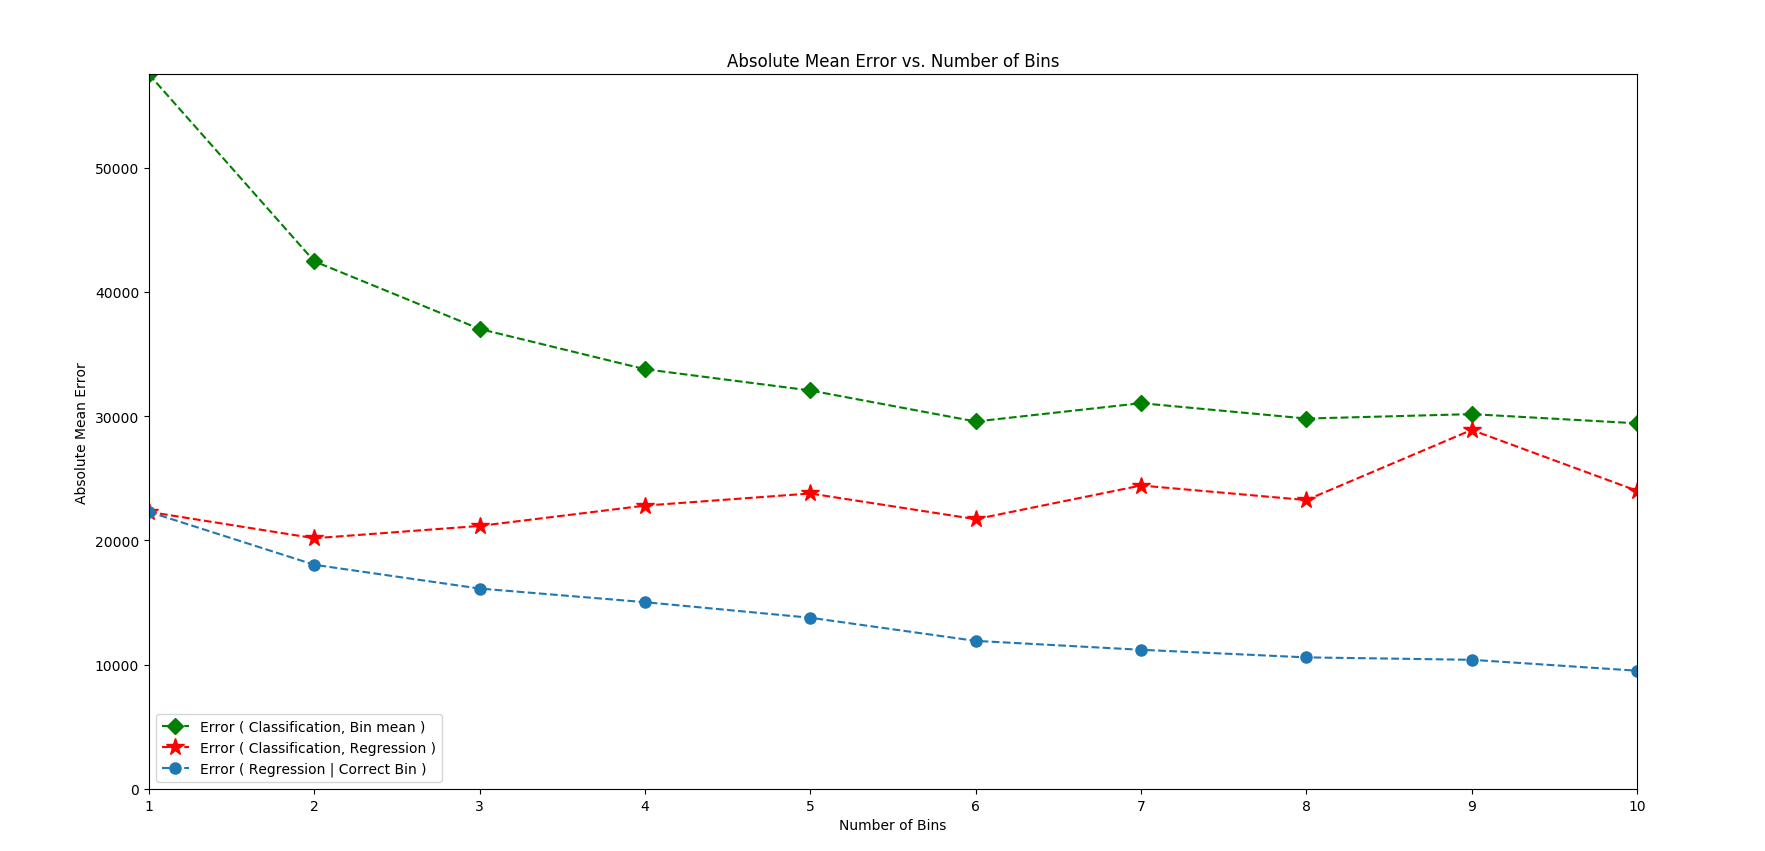
\includegraphics[width=\linewidth,natwidth=1765,natheight=851]{Decisiontree_linear_lines.png}
  \caption{Custom Model Training - Regression Errors vs. Number of Bins}
  \label{fig:regressionerror}
\end{figure*}

\par
The training process provides the ideal number of bins and the validation error of the custom model (the red curve in Fig. \ref{fig:regressionerror}). We separately kept track of the classification error (Fig. \ref{fig:classificatinerror}) and regression error, given correct bin labels (the blue curve in Fig. \ref{fig:regressionerror}) to peek inside the custom model to see what is working right and what is not. The blue curve provides a lower bound to the model. Options to try to get a error below the blue curve are finding a better regression model, feature engineering or obtaining a better feature set.

\par
We further keep track of the error if we predict bin average as the prediction (green curve in Fig. \ref{fig:regressionerror}) . This provides an upper bound for the error.

%We used the bin average as a prediction to house prices in all the houses that fall into a single bin to gauge how well the model is working. With bin average as the prediction we kept track of custom model error and the error given the correct bin. These errors provide an upper bound for the model.

\subsubsection{Custom Model - Experiments:} 
\par
Our initial choice for the classifier-regressor pair for the custom model was decision trees and linear regression (Fig. \ref{fig:customDtLr}).

\begin{figure}[!h]
  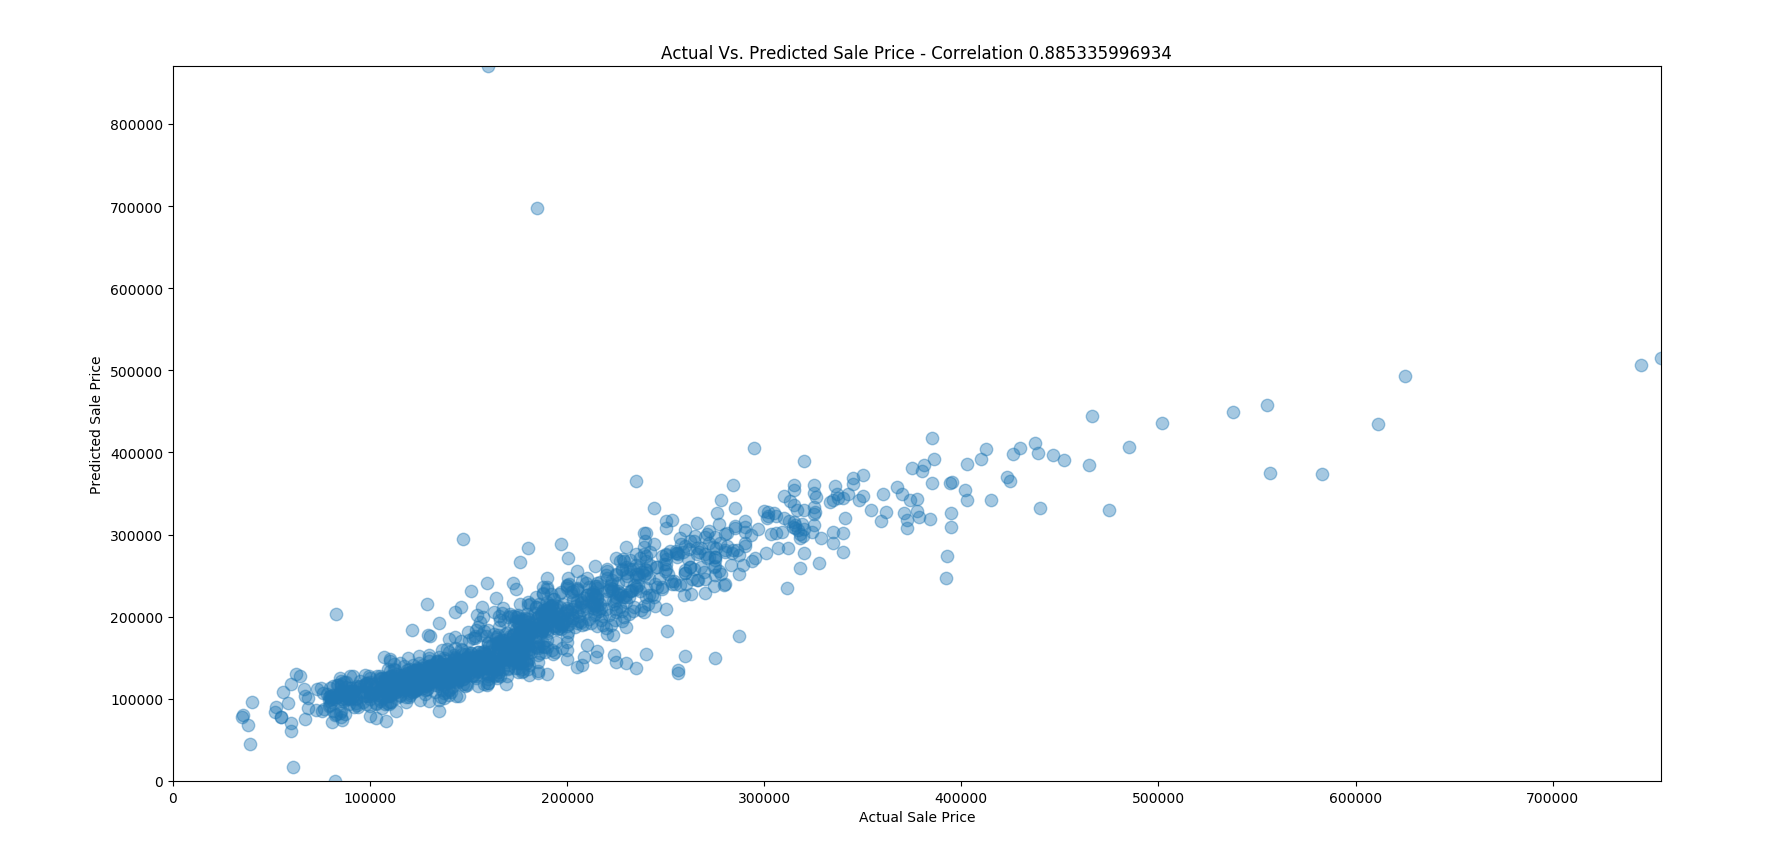
\includegraphics[width=\linewidth,natwidth=1179,natheight=853]{Decisiontree_linear_scatter2bins.png}
  \caption{Custom Model Decision Trees + Linear Regression - Actual vs. Predicted Sale Price}
  \label{fig:customDtLr}
\end{figure}



\section{Error Analysis:}
As we can see from the graph in Fig. \ref{fig:regressionerror}, the difference between the blue and red curves denotes the area our model can improve on for better prediction. As the complex model consists of the two stages: the classification and regression stage, we can attempt to improve either or both of them. However, from our previous experiments, we know that the regression models perform quite well on the numeric and ordinal attributes, which indicates that the classification stage has potential for improvement. The further proof of this is shown in Fig. \ref{fig:customDtLr}, which shows decision tree classifier and linear regression to have a correlation of 0.881, with an optimum bin number of 2 bins. This correlation is lower than the correlation of 0.917 when using simple linear regression on only linear and ordinal attributes. We contribute the reduction in performance to incorrect classification of houses into bins, or incorrect binning scheme, which are both part of the classification stage. Therefore, we tried two methods to improve the classification stage.

\begin{itemize}
\par
\item \textit {Different Classification Algorithm: } Given the binning scheme, it is possible the existing classification algorithm is not able to learn the association between attributes of houses and the assigned bin labels well. Therefore, a different classifier might be able to learn the binning better, resulting in coherent bins, which in turn improves the accuracy of our regression stage.
\item \textit {Different Binning Scheme: } It is also possible that the existing binning scheme does not give rise to a learnable pattern between feature vectors and assigned bin labels. This renders any classifier hopeless. Therefore, a different binning scheme, which bins homogeneous houses into a single bin, can also improve performance.
\end{itemize}


\section {Improved Custom Model}

\begin{table*}[!htbp]
\centering
\caption{Custom Model - Errors and Correlations}
\label{table:custommodperf}
\begin{tabular}{llll}
                                                                   & Mean Absolute Error & Correlation & Optimal Bins\\
Decision Tree \& Linear Regression                                 & 20,283              & 0.881       & 2\\
Random Forest Classifier \& Regression                             & 19,279              & 0.910       & 1\\
Gradient Boosting Classifier \& Regression                         & 17,957              & 0.921       & 2\\
K-means, Decision Tree \& Linear Regression                        & 22,393              & 0.867       & 1\\
Gaussian Mixture Model, Decision Tree \& Linear Regression         & 22,429              & 0.867       & 1\\
K-means, Gradient Boosting Classifier \& Regression                & 18,201              & 0.919       & 2\\
Gaussian Mixture Model, Gradient Boosting Classifier \& Regression & 17,853              & 0.921       & 2
\end{tabular}
\end{table*}




We tried different models for each of the possible options mentioned above.

\subsection {Different Classification Algorithm}
We tried several different classification algorithms. We also tried different combinations of classifier and regression models. Since Gradient Boosting and Random Forest regressors worked well in the regression models, we decided to attempt gradient boosting and random forest classification and regression models together. Table \ref{table:custommodperf} shows the correlation for each of the models.
As we can see, Gradient Boosting Classifier and Regressor model perform the best with a correlation of 0.921, with an optimum bin number of 2 bins, which is close to the best model of using simple gradient boosting regressor model, which had a correlation of 0.947, and also an improvement from our original custom model. 

\subsection {Different Binning Schemes}
Given that we are using equal frequency bins in the original model, it is possible that houses which are significantly different from each other could be put in the same bin, which could be the reason that decreases the accuracy of our classification models. This is especially true for the last bin as there are very few houses with high sale prices, these houses might be put in the same bin as some significantly lower priced houses. Therefore we hypothesize, a scheme which forms more coherent bins where the differences in the houses that fall within one bin are not as significant as equal frequency binning can improve binning. Following this logic, we decided to try K-means clustering and Gaussian Mixture Models to do binning, which are then fed to the classifier. We attempted four different combinations, which are

\begin {itemize}
  \item K-means clustering with Decision Tree Classifier and Linear Regressor
  \item Gaussian Mixture Model with Decision Tree Classifier and Linear Regressor
  \item K-means Clustering with Gradient Boosting Classifier and Regressor
  \item Gaussian Mixture Model with Gradient Boosting Classifier and Regressor
\end{itemize} 

\par
We decided to attempt gradient boosting as well, as it is the best performing classifier and regressor thus far. Table \ref{table:custommodperf} shows the performances of these four models.
Both k-means and Gaussian Mixture Models with decision tree classifier and linear regression achieve a correlation of 0.867, which is an improvement from our original model. K-means and Gaussian Mixture Models with gradient boosting classifier and regressor achieve a correlation of 0.921, which is close to our best model.

\par
Both K-means clustering and Gaussian Mixture Models based bin assignment strategies give almost identical results. Gaussian Mixture Models is a generalization of K-means clustering. So, the bin assignments provided by both of them are comparable, which is the reason behind this observation. This leads to the conclusion that employing more complex Gaussian Mixture Models for bin assignment does not add any value for the system.


\section {Discussion}
\begin{figure}[!h]
  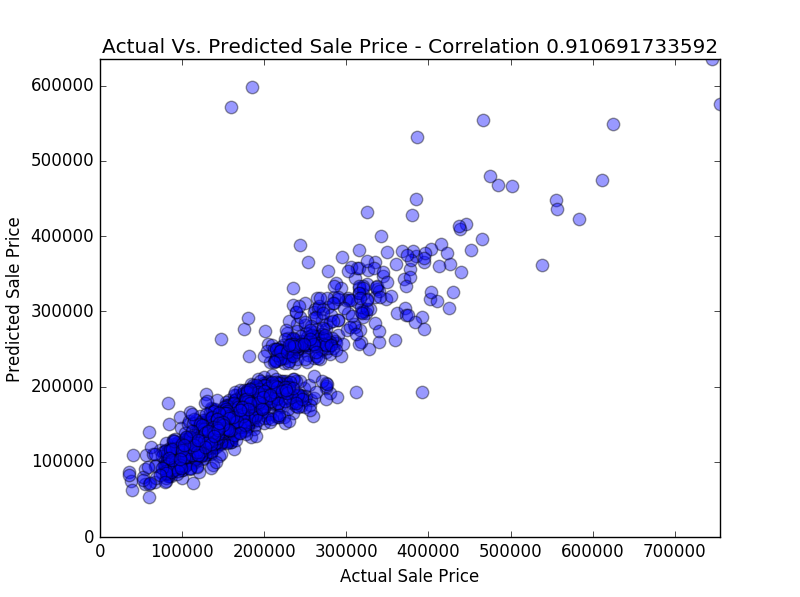
\includegraphics[width=\linewidth,natwidth=800,natheight=597]{bin2kmeansrf.png}
  \caption{Effect of Binning on Regression Prediction - 2 Bins}
  \label{fig:binningeffect}
\end{figure}

\begin{figure}[!h]
  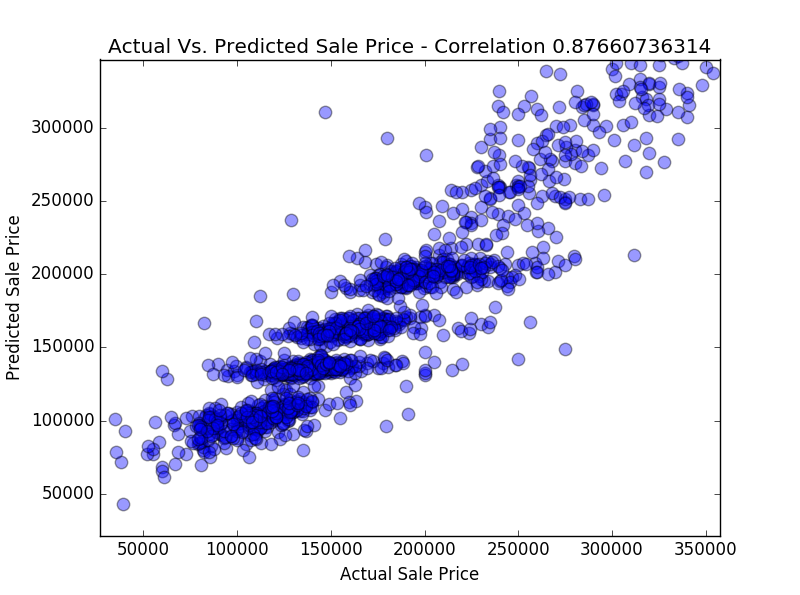
\includegraphics[width=\linewidth,natwidth=800,natheight=597]{Stairecase.png}
  \caption{Effect of Binning on Regression Prediction - 5 Bins}
  \label{fig:binningeffect2}
\end{figure}


\par
From our results, we observe different classification algorithms and binning schemes both improve the performance of the original custom model with Decision Trees and Linear Regression, and the use of ensembles significantly improve the accuracy of the models. 

\par
However, according to the table \ref{table:custommodperf}, the optimal number of bins for the the best performing models is one with Gradient Boosting Classifier being the only exception. This is also due to the fact that the Gradient Boosting Classifier does not work with a single class. Furthermore, comparing the results of the simple model which uses just the Gradient Boosting Regressor with the custom model which uses Gradient Boosting Classifier and Regressor, we observed that the simple model performs better.%just using the Gradient Boosting Regressor works better.

\par
Custom model with a single bin means that the classifier does not add any improvement and it is equivalent to a simple model with only the regressor. Based on this observation, we can conclude, the custom model we have thus far fails to improve beyond the best results we get with a simple model.

\par
Regressor versions of the ensemble models are built upon the classifier version of the respective models. This could most probably be the reason why when ensemble model classifier and regressor pairs plugged into custom model not being able to outperform directly using the regressor version of the ensemble models. 


\par
Moreover, in the custom model, a misclassification in the bin prediction level is very costly since the final price will be predicted based on a regression model totally irrelevant to that house. The further the predicted bin is from the actual bin, the more the error. With the direct regression models, such effect could be mild since we estimate the house price based on a model trained on all the houses.

\par
This phenomenon is visible in the scatter plot in Figure \ref{fig:binningeffect} and \ref{fig:binningeffect2} having two visible clusters, which are for the two bins that the respective model used to make the predictions on. With higher number of bins a staircase like clustering is visible in the actual vs. predicted price scatter plot with number of clusters equal to the number of bins.

\par
In our present implementation, we segment the training examples into bins in a strictly non-overlapping manner and train the regression models on those bins (bin b contains only the examples labeled with bin b). The staircase effect (Fig. \ref{fig:binningeffect2}) in the scatter plots suggests that this assignment introduces discontinuities into the fitted model. We suggest introducing a overlapping factor into the model so that the examples are segmented into bins in an overlapping manner (bin b also contains some examples with higher sale prices labeled bin b-1 and some examples with lower sale prices labeled bin b+1). This would introduce a smoothing effect into individual regression model training and consequently alleviate the staircase effect. In this regard, the present model has zero overlapping factor. Higher the overlapping factor, closer each regression model to a regression model trained without any binning.


\section {Conclusion}
We started our investigation on the Kaggle housing price data by carrying out some feature manipulation and selecting and running simple regression models. Here we observed, ensemble models, especially gradient boosting worked best when using all attributes and linear regressor performed close to it using only numeric and ordinal attributes, which gave way to two research question.

\par
We were able to answer the first research question by building a custom model using a combination of a classifier and regression model. We also improved the custom model by introducing the use of different classification algorithms and binning schemes.

\par
The custom model was able to slightly improve the performance of Linear and Lasso regression. However, it failed to add any improvement to ensemble models.

\par
More feature engineering with the aid of domain knowledge, further investigation into defining better binning and bin classification algorithms are the future directions that we can take to improve the prediction accuracy of this problem.

%\par
%(I think we have to remove this part)
%The performance of our improved model were close to our best achieved performance from all models, which answered our second research question. We believe more intuitive feature selection and other classification and binning approaches will be able to improve the performance of our custom model. 


% An example of a floating figure using the graphicx package.
% Note that \label must occur AFTER (or within) \caption.
% For figures, \caption should occur after the \includegraphics.
% Note that IEEEtran v1.7 and later has special internal code that
% is designed to preserve the operation of \label within \caption
% even when the captionsoff option is in effect. However, because
% of issues like this, it may be the safest practice to put all your
% \label just after \caption rather than within \caption{}.
%
% Reminder: the "draftcls" or "draftclsnofoot", not "draft", class
% option should be used if it is desired that the figures are to be
% displayed while in draft mode.
%
%\begin{figure}[!t]
%\centering
%\includegraphics[width=2.5in]{myfigure}
% where an .eps filename suffix will be assumed under latex, 
% and a .pdf suffix will be assumed for pdflatex; or what has been declared
% via \DeclareGraphicsExtensions.
%\caption{Simulation results for the network.}
%\label{fig_sim}
%\end{figure}

% Note that the IEEE typically puts floats only at the top, even when this
% results in a large percentage of a column being occupied by floats.


% An example of a double column floating figure using two subfigures.
% (The subfig.sty package must be loaded for this to work.)
% The subfigure \label commands are set within each subfloat command,
% and the \label for the overall figure must come after \caption.
% \hfil is used as a separator to get equal spacing.
% Watch out that the combined width of all the subfigures on a 
% line do not exceed the text width or a line break will occur.
%
%\begin{figure*}[!t]
%\centering
%\subfloat[Case I]{\includegraphics[width=2.5in]{box}%
%\label{fig_first_case}}
%\hfil
%\subfloat[Case II]{\includegraphics[width=2.5in]{box}%
%\label{fig_second_case}}
%\caption{Simulation results for the network.}
%\label{fig_sim}
%\end{figure*}
%
% Note that often IEEE papers with subfigures do not employ subfigure
% captions (using the optional argument to \subfloat[]), but instead will
% reference/describe all of them (a), (b), etc., within the main caption.
% Be aware that for subfig.sty to generate the (a), (b), etc., subfigure
% labels, the optional argument to \subfloat must be present. If a
% subcaption is not desired, just leave its contents blank,
% e.g., \subfloat[].


% An example of a floating table. Note that, for IEEE style tables, the
% \caption command should come BEFORE the table and, given that table
% captions serve much like titles, are usually capitalized except for words
% such as a, an, and, as, at, but, by, for, in, nor, of, on, or, the, to
% and up, which are usually not capitalized unless they are the first or
% last word of the caption. Table text will default to \footnotesize as
% the IEEE normally uses this smaller font for tables.
% The \label must come after \caption as always.
%
%\begin{table}[!t]
%% increase table row spacing, adjust to taste
%\renewcommand{\arraystretch}{1.3}
% if using array.sty, it might be a good idea to tweak the value of
% \extrarowheight as needed to properly center the text within the cells
%\caption{An Example of a Table}
%\label{table_example}
%\centering
%% Some packages, such as MDW tools, offer better commands for making tables
%% than the plain LaTeX2e tabular which is used here.
%\begin{tabular}{|c||c|}
%\hline
%One & Two\\
%\hline
%Three & Four\\
%\hline
%\end{tabular}
%\end{table}


% Note that the IEEE does not put floats in the very first column
% - or typically anywhere on the first page for that matter. Also,
% in-text middle ("here") positioning is typically not used, but it
% is allowed and encouraged for Computer Society conferences (but
% not Computer Society journals). Most IEEE journals/conferences use
% top floats exclusively. 
% Note that, LaTeX2e, unlike IEEE journals/conferences, places
% footnotes above bottom floats. This can be corrected via the
% \fnbelowfloat command of the stfloats package.


% conference papers do not normally have an appendix



% use section* for acknowledgment
%\ifCLASSOPTIONcompsoc
  % The Computer Society usually uses the plural form
%  \section*{Acknowledgments}
%\else
  % regular IEEE prefers the singular form
%  \section*{Acknowledgment}
%\fi


%The authors would like to thank...





% trigger a \newpage just before the given reference
% number - used to balance the columns on the last page
% adjust value as needed - may need to be readjusted if
% the document is modified later
%\IEEEtriggeratref{8}
% The "triggered" command can be changed if desired:
%\IEEEtriggercmd{\enlargethispage{-5in}}

% references section

% can use a bibliography generated by BibTeX as a .bbl file
% BibTeX documentation can be easily obtained at:
% http://mirror.ctan.org/biblio/bibtex/contrib/doc/
% The IEEEtran BibTeX style support page is at:
% http://www.michaelshell.org/tex/ieeetran/bibtex/
%\bibliographystyle{IEEEtran}
% argument is your BibTeX string definitions and bibliography database(s)
%\bibliography{IEEEabrv,../bib/paper}
%
% <OR> manually copy in the resultant .bbl file
% set second argument of \begin to the number of references
% (used to reserve space for the reference number labels box)
%\begin{thebibliography}{1}

%\bibitem{IEEEhowto:kopka}
%H.~Kopka and P.~W. Daly, \emph{A Guide to \LaTeX}, 3rd~ed.\hskip 1em plus
%  0.5em minus 0.4em\relax Harlow, England: Addison-Wesley, 1999.

%\end{thebibliography}




% that's all folks
\end{document}


